\documentclass[twoside]{book}

% Packages required by doxygen
\usepackage{fixltx2e}
\usepackage{calc}
\usepackage{doxygen}
\usepackage[export]{adjustbox} % also loads graphicx
\usepackage{graphicx}
\usepackage[utf8]{inputenc}
\usepackage{makeidx}
\usepackage{multicol}
\usepackage{multirow}
\PassOptionsToPackage{warn}{textcomp}
\usepackage{textcomp}
\usepackage[nointegrals]{wasysym}
\usepackage[table]{xcolor}

% Font selection
\usepackage[T1]{fontenc}
\usepackage[scaled=.90]{helvet}
\usepackage{courier}
\usepackage{amssymb}
\usepackage{sectsty}
\renewcommand{\familydefault}{\sfdefault}
\allsectionsfont{%
  \fontseries{bc}\selectfont%
  \color{darkgray}%
}
\renewcommand{\DoxyLabelFont}{%
  \fontseries{bc}\selectfont%
  \color{darkgray}%
}
\newcommand{\+}{\discretionary{\mbox{\scriptsize$\hookleftarrow$}}{}{}}

% Page & text layout
\usepackage{geometry}
\geometry{%
  a4paper,%
  top=2.5cm,%
  bottom=2.5cm,%
  left=2.5cm,%
  right=2.5cm%
}
\tolerance=750
\hfuzz=15pt
\hbadness=750
\setlength{\emergencystretch}{15pt}
\setlength{\parindent}{0cm}
\setlength{\parskip}{3ex plus 2ex minus 2ex}
\makeatletter
\renewcommand{\paragraph}{%
  \@startsection{paragraph}{4}{0ex}{-1.0ex}{1.0ex}{%
    \normalfont\normalsize\bfseries\SS@parafont%
  }%
}
\renewcommand{\subparagraph}{%
  \@startsection{subparagraph}{5}{0ex}{-1.0ex}{1.0ex}{%
    \normalfont\normalsize\bfseries\SS@subparafont%
  }%
}
\makeatother

% Headers & footers
\usepackage{fancyhdr}
\pagestyle{fancyplain}
\fancyhead[LE]{\fancyplain{}{\bfseries\thepage}}
\fancyhead[CE]{\fancyplain{}{}}
\fancyhead[RE]{\fancyplain{}{\bfseries\leftmark}}
\fancyhead[LO]{\fancyplain{}{\bfseries\rightmark}}
\fancyhead[CO]{\fancyplain{}{}}
\fancyhead[RO]{\fancyplain{}{\bfseries\thepage}}
\fancyfoot[LE]{\fancyplain{}{}}
\fancyfoot[CE]{\fancyplain{}{}}
\fancyfoot[RE]{\fancyplain{}{\bfseries\scriptsize Generated by Doxygen }}
\fancyfoot[LO]{\fancyplain{}{\bfseries\scriptsize Generated by Doxygen }}
\fancyfoot[CO]{\fancyplain{}{}}
\fancyfoot[RO]{\fancyplain{}{}}
\renewcommand{\footrulewidth}{0.4pt}
\renewcommand{\chaptermark}[1]{%
  \markboth{#1}{}%
}
\renewcommand{\sectionmark}[1]{%
  \markright{\thesection\ #1}%
}

% Indices & bibliography
\usepackage{natbib}
\usepackage[titles]{tocloft}
\setcounter{tocdepth}{3}
\setcounter{secnumdepth}{5}
\makeindex

% Hyperlinks (required, but should be loaded last)
\usepackage{ifpdf}
\ifpdf
  \usepackage[pdftex,pagebackref=true]{hyperref}
\else
  \usepackage[ps2pdf,pagebackref=true]{hyperref}
\fi
\hypersetup{%
  colorlinks=true,%
  linkcolor=blue,%
  citecolor=blue,%
  unicode%
}

% Custom commands
\newcommand{\clearemptydoublepage}{%
  \newpage{\pagestyle{empty}\cleardoublepage}%
}

\usepackage{caption}
\captionsetup{labelsep=space,justification=centering,font={bf},singlelinecheck=off,skip=4pt,position=top}

%===== C O N T E N T S =====

\begin{document}

% Titlepage & ToC
\hypersetup{pageanchor=false,
             bookmarksnumbered=true,
             pdfencoding=unicode
            }
\pagenumbering{alph}
\begin{titlepage}
\vspace*{7cm}
\begin{center}%
{\Large Ogród zoologiczny }\\
\vspace*{1cm}
{\large Generated by Doxygen 1.8.14}\\
\end{center}
\end{titlepage}
\clearemptydoublepage
\pagenumbering{roman}
\tableofcontents
\clearemptydoublepage
\pagenumbering{arabic}
\hypersetup{pageanchor=true}

%--- Begin generated contents ---
\chapter{Data Structure Index}
\section{Data Structures}
Here are the data structures with brief descriptions\+:\begin{DoxyCompactList}
\item\contentsline{section}{\mbox{\hyperlink{struct_http_response}{Http\+Response}} }{\pageref{struct_http_response}}{}
\end{DoxyCompactList}

\chapter{File Index}
\section{File List}
Here is a list of all files with brief descriptions\+:\begin{DoxyCompactList}
\item\contentsline{section}{include/\mbox{\hyperlink{main__window_8h}{main\+\_\+window.\+h}} }{\pageref{main__window_8h}}{}
\item\contentsline{section}{include/services/\mbox{\hyperlink{http_8h}{http.\+h}} }{\pageref{http_8h}}{}
\item\contentsline{section}{src/\mbox{\hyperlink{main_8c}{main.\+c}} }{\pageref{main_8c}}{}
\item\contentsline{section}{src/\mbox{\hyperlink{main__window_8c}{main\+\_\+window.\+c}} }{\pageref{main__window_8c}}{}
\item\contentsline{section}{src/services/\mbox{\hyperlink{http_8c}{http.\+c}} }{\pageref{http_8c}}{}
\end{DoxyCompactList}

\chapter{Data Structure Documentation}
\hypertarget{struct_http_response}{}\section{Http\+Response Struct Reference}
\label{struct_http_response}\index{Http\+Response@{Http\+Response}}


{\ttfamily \#include $<$http.\+h$>$}



Collaboration diagram for Http\+Response\+:\nopagebreak
\begin{figure}[H]
\begin{center}
\leavevmode
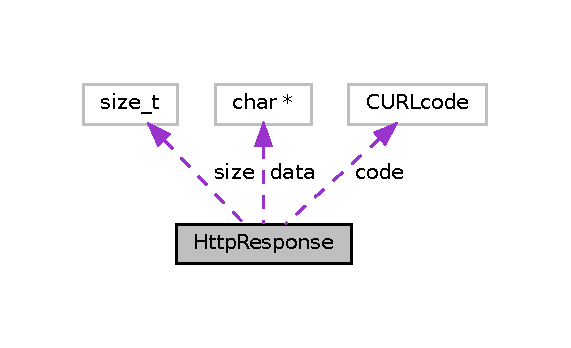
\includegraphics[width=274pt]{struct_http_response__coll__graph}
\end{center}
\end{figure}
\subsection*{Data Fields}
\begin{DoxyCompactItemize}
\item 
char $\ast$ \mbox{\hyperlink{struct_http_response_a29b7ecfb11da1af6c7fdd3fe7862901f}{data}}
\item 
size\+\_\+t \mbox{\hyperlink{struct_http_response_a11b910682b365528a15fcfd6d4dd824f}{size}}
\item 
C\+U\+R\+Lcode \mbox{\hyperlink{struct_http_response_abce68ae6776a536dce762f0b6a96ab54}{code}}
\end{DoxyCompactItemize}


\subsection{Detailed Description}


Definition at line 8 of file http.\+h.



\subsection{Field Documentation}
\mbox{\Hypertarget{struct_http_response_abce68ae6776a536dce762f0b6a96ab54}\label{struct_http_response_abce68ae6776a536dce762f0b6a96ab54}} 
\index{Http\+Response@{Http\+Response}!code@{code}}
\index{code@{code}!Http\+Response@{Http\+Response}}
\subsubsection{\texorpdfstring{code}{code}}
{\footnotesize\ttfamily C\+U\+R\+Lcode Http\+Response\+::code}



Definition at line 11 of file http.\+h.



Referenced by http\+\_\+get().

\mbox{\Hypertarget{struct_http_response_a29b7ecfb11da1af6c7fdd3fe7862901f}\label{struct_http_response_a29b7ecfb11da1af6c7fdd3fe7862901f}} 
\index{Http\+Response@{Http\+Response}!data@{data}}
\index{data@{data}!Http\+Response@{Http\+Response}}
\subsubsection{\texorpdfstring{data}{data}}
{\footnotesize\ttfamily char$\ast$ Http\+Response\+::data}



Definition at line 9 of file http.\+h.



Referenced by http\+\_\+get(), http\+\_\+response\+\_\+new(), and write\+\_\+function().

\mbox{\Hypertarget{struct_http_response_a11b910682b365528a15fcfd6d4dd824f}\label{struct_http_response_a11b910682b365528a15fcfd6d4dd824f}} 
\index{Http\+Response@{Http\+Response}!size@{size}}
\index{size@{size}!Http\+Response@{Http\+Response}}
\subsubsection{\texorpdfstring{size}{size}}
{\footnotesize\ttfamily size\+\_\+t Http\+Response\+::size}



Definition at line 10 of file http.\+h.



Referenced by http\+\_\+response\+\_\+new(), and write\+\_\+function().



The documentation for this struct was generated from the following file\+:\begin{DoxyCompactItemize}
\item 
include/services/\mbox{\hyperlink{http_8h}{http.\+h}}\end{DoxyCompactItemize}

\chapter{File Documentation}
\hypertarget{main__window_8h}{}\section{include/main\+\_\+window.h File Reference}
\label{main__window_8h}\index{include/main\+\_\+window.\+h@{include/main\+\_\+window.\+h}}
{\ttfamily \#include $<$gtk/gtk.\+h$>$}\newline
{\ttfamily \#include \char`\"{}data/animal.\+h\char`\"{}}\newline
Include dependency graph for main\+\_\+window.\+h\+:
\nopagebreak
\begin{figure}[H]
\begin{center}
\leavevmode
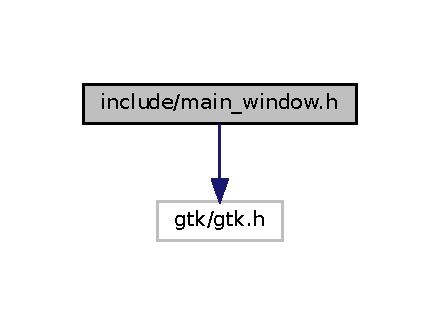
\includegraphics[width=242pt]{main__window_8h__incl}
\end{center}
\end{figure}
This graph shows which files directly or indirectly include this file\+:
\nopagebreak
\begin{figure}[H]
\begin{center}
\leavevmode
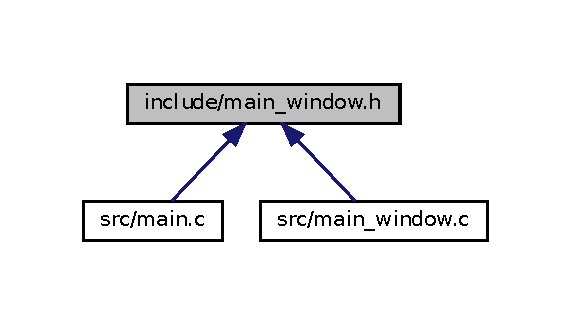
\includegraphics[width=274pt]{main__window_8h__dep__incl}
\end{center}
\end{figure}
\subsection*{Data Structures}
\begin{DoxyCompactItemize}
\item 
struct \mbox{\hyperlink{struct_sort_callback_data}{Sort\+Callback\+Data}}
\end{DoxyCompactItemize}
\subsection*{Typedefs}
\begin{DoxyCompactItemize}
\item 
typedef enum \mbox{\hyperlink{main__window_8h_a727e9b9696032b380d0072840595ef05}{C\+O\+L\+U\+MN}} \mbox{\hyperlink{main__window_8h_a59f2ba426d7dcdfd9ade0a53aa7ee628}{C\+O\+L\+U\+MN}}
\item 
typedef struct \mbox{\hyperlink{struct_sort_callback_data}{Sort\+Callback\+Data}} \mbox{\hyperlink{main__window_8h_a96108b6df1df3189b7dd150e27a920db}{Sort\+Callback\+Data}}
\end{DoxyCompactItemize}
\subsection*{Enumerations}
\begin{DoxyCompactItemize}
\item 
enum \mbox{\hyperlink{main__window_8h_a727e9b9696032b380d0072840595ef05}{C\+O\+L\+U\+MN}} \{ \newline
\mbox{\hyperlink{main__window_8h_a727e9b9696032b380d0072840595ef05a001479a58fb44c39a29b20d565081a68}{ID}}, 
\mbox{\hyperlink{main__window_8h_a727e9b9696032b380d0072840595ef05a67bc2ced260a8e43805d2480a785d312}{N\+A\+ME}}, 
\mbox{\hyperlink{main__window_8h_a727e9b9696032b380d0072840595ef05a1663380252e067c51dd9ccc2b765691f}{S\+P\+E\+C\+I\+ES}}, 
\mbox{\hyperlink{main__window_8h_a727e9b9696032b380d0072840595ef05a9fc6b2c465e5d1c9e839400fa1e1dfbc}{A\+GE}}, 
\newline
\mbox{\hyperlink{main__window_8h_a727e9b9696032b380d0072840595ef05aae696377c19e507b64e16be78ce3bbdb}{C\+O\+M\+M\+E\+NT}}
 \}
\end{DoxyCompactItemize}
\subsection*{Functions}
\begin{DoxyCompactItemize}
\item 
Gtk\+Widget $\ast$ \mbox{\hyperlink{main__window_8h_adcf0e83db47ee039761c9b42887a6c6c}{main\+\_\+window\+\_\+new}} (Gtk\+Application $\ast$app)
\begin{DoxyCompactList}\small\item\em Initialize the main window. \end{DoxyCompactList}\item 
void \mbox{\hyperlink{main__window_8h_a14991586378d572e198ab90004e60e5d}{callback\+\_\+sort\+\_\+click}} (Gtk\+Widget $\ast$widget, gpointer callback\+\_\+data)
\item 
void \mbox{\hyperlink{main__window_8h_af1eaf0a9c2a7070f525386bb7ef4bac0}{add\+\_\+table\+\_\+headers}} (Gtk\+Widget $\ast$main\+Container, Gtk\+Widget $\ast$table, \mbox{\hyperlink{struct_animal_linked_list}{Animal\+Linked\+List}} $\ast$animals)
\begin{DoxyCompactList}\small\item\em Add table header buttons. \end{DoxyCompactList}\item 
void \mbox{\hyperlink{main__window_8h_acb8a7744ef425d1083a95017a3eaf1d7}{add\+\_\+control\+\_\+buttons}} (Gtk\+Application $\ast$app, Gtk\+Widget $\ast$main\+Container)
\item 
void \mbox{\hyperlink{main__window_8h_a7cd8ebd9f8b95eb48255fa9217843ca7}{fill\+\_\+table}} (Gtk\+Widget $\ast$table, \mbox{\hyperlink{struct_animal_linked_list}{Animal\+Linked\+List}} $\ast$animals)
\end{DoxyCompactItemize}


\subsection{Typedef Documentation}
\mbox{\Hypertarget{main__window_8h_a59f2ba426d7dcdfd9ade0a53aa7ee628}\label{main__window_8h_a59f2ba426d7dcdfd9ade0a53aa7ee628}} 
\index{main\+\_\+window.\+h@{main\+\_\+window.\+h}!C\+O\+L\+U\+MN@{C\+O\+L\+U\+MN}}
\index{C\+O\+L\+U\+MN@{C\+O\+L\+U\+MN}!main\+\_\+window.\+h@{main\+\_\+window.\+h}}
\subsubsection{\texorpdfstring{C\+O\+L\+U\+MN}{COLUMN}}
{\footnotesize\ttfamily typedef enum \mbox{\hyperlink{main__window_8h_a727e9b9696032b380d0072840595ef05}{C\+O\+L\+U\+MN}}
         \mbox{\hyperlink{main__window_8h_a727e9b9696032b380d0072840595ef05}{C\+O\+L\+U\+MN}}}

\mbox{\Hypertarget{main__window_8h_a96108b6df1df3189b7dd150e27a920db}\label{main__window_8h_a96108b6df1df3189b7dd150e27a920db}} 
\index{main\+\_\+window.\+h@{main\+\_\+window.\+h}!Sort\+Callback\+Data@{Sort\+Callback\+Data}}
\index{Sort\+Callback\+Data@{Sort\+Callback\+Data}!main\+\_\+window.\+h@{main\+\_\+window.\+h}}
\subsubsection{\texorpdfstring{Sort\+Callback\+Data}{SortCallbackData}}
{\footnotesize\ttfamily typedef struct \mbox{\hyperlink{struct_sort_callback_data}{Sort\+Callback\+Data}}  \mbox{\hyperlink{struct_sort_callback_data}{Sort\+Callback\+Data}}}



\subsection{Enumeration Type Documentation}
\mbox{\Hypertarget{main__window_8h_a727e9b9696032b380d0072840595ef05}\label{main__window_8h_a727e9b9696032b380d0072840595ef05}} 
\index{main\+\_\+window.\+h@{main\+\_\+window.\+h}!C\+O\+L\+U\+MN@{C\+O\+L\+U\+MN}}
\index{C\+O\+L\+U\+MN@{C\+O\+L\+U\+MN}!main\+\_\+window.\+h@{main\+\_\+window.\+h}}
\subsubsection{\texorpdfstring{C\+O\+L\+U\+MN}{COLUMN}}
{\footnotesize\ttfamily enum \mbox{\hyperlink{main__window_8h_a727e9b9696032b380d0072840595ef05}{C\+O\+L\+U\+MN}}}

\begin{DoxyEnumFields}{Enumerator}
\raisebox{\heightof{T}}[0pt][0pt]{\index{ID@{ID}!main\+\_\+window.\+h@{main\+\_\+window.\+h}}\index{main\+\_\+window.\+h@{main\+\_\+window.\+h}!ID@{ID}}}\mbox{\Hypertarget{main__window_8h_a727e9b9696032b380d0072840595ef05a001479a58fb44c39a29b20d565081a68}\label{main__window_8h_a727e9b9696032b380d0072840595ef05a001479a58fb44c39a29b20d565081a68}} 
ID&\\
\hline

\raisebox{\heightof{T}}[0pt][0pt]{\index{N\+A\+ME@{N\+A\+ME}!main\+\_\+window.\+h@{main\+\_\+window.\+h}}\index{main\+\_\+window.\+h@{main\+\_\+window.\+h}!N\+A\+ME@{N\+A\+ME}}}\mbox{\Hypertarget{main__window_8h_a727e9b9696032b380d0072840595ef05a67bc2ced260a8e43805d2480a785d312}\label{main__window_8h_a727e9b9696032b380d0072840595ef05a67bc2ced260a8e43805d2480a785d312}} 
N\+A\+ME&\\
\hline

\raisebox{\heightof{T}}[0pt][0pt]{\index{S\+P\+E\+C\+I\+ES@{S\+P\+E\+C\+I\+ES}!main\+\_\+window.\+h@{main\+\_\+window.\+h}}\index{main\+\_\+window.\+h@{main\+\_\+window.\+h}!S\+P\+E\+C\+I\+ES@{S\+P\+E\+C\+I\+ES}}}\mbox{\Hypertarget{main__window_8h_a727e9b9696032b380d0072840595ef05a1663380252e067c51dd9ccc2b765691f}\label{main__window_8h_a727e9b9696032b380d0072840595ef05a1663380252e067c51dd9ccc2b765691f}} 
S\+P\+E\+C\+I\+ES&\\
\hline

\raisebox{\heightof{T}}[0pt][0pt]{\index{A\+GE@{A\+GE}!main\+\_\+window.\+h@{main\+\_\+window.\+h}}\index{main\+\_\+window.\+h@{main\+\_\+window.\+h}!A\+GE@{A\+GE}}}\mbox{\Hypertarget{main__window_8h_a727e9b9696032b380d0072840595ef05a9fc6b2c465e5d1c9e839400fa1e1dfbc}\label{main__window_8h_a727e9b9696032b380d0072840595ef05a9fc6b2c465e5d1c9e839400fa1e1dfbc}} 
A\+GE&\\
\hline

\raisebox{\heightof{T}}[0pt][0pt]{\index{C\+O\+M\+M\+E\+NT@{C\+O\+M\+M\+E\+NT}!main\+\_\+window.\+h@{main\+\_\+window.\+h}}\index{main\+\_\+window.\+h@{main\+\_\+window.\+h}!C\+O\+M\+M\+E\+NT@{C\+O\+M\+M\+E\+NT}}}\mbox{\Hypertarget{main__window_8h_a727e9b9696032b380d0072840595ef05aae696377c19e507b64e16be78ce3bbdb}\label{main__window_8h_a727e9b9696032b380d0072840595ef05aae696377c19e507b64e16be78ce3bbdb}} 
C\+O\+M\+M\+E\+NT&\\
\hline

\end{DoxyEnumFields}


Definition at line 24 of file main\+\_\+window.\+h.


\begin{DoxyCode}
24                     \{\mbox{\hyperlink{main__window_8h_a727e9b9696032b380d0072840595ef05a001479a58fb44c39a29b20d565081a68}{ID}},
25     \mbox{\hyperlink{main__window_8h_a727e9b9696032b380d0072840595ef05a67bc2ced260a8e43805d2480a785d312}{NAME}},
26     \mbox{\hyperlink{main__window_8h_a727e9b9696032b380d0072840595ef05a1663380252e067c51dd9ccc2b765691f}{SPECIES}},
27     \mbox{\hyperlink{main__window_8h_a727e9b9696032b380d0072840595ef05a9fc6b2c465e5d1c9e839400fa1e1dfbc}{AGE}},
28     \mbox{\hyperlink{main__window_8h_a727e9b9696032b380d0072840595ef05aae696377c19e507b64e16be78ce3bbdb}{COMMENT}}\}
\end{DoxyCode}


\subsection{Function Documentation}
\mbox{\Hypertarget{main__window_8h_acb8a7744ef425d1083a95017a3eaf1d7}\label{main__window_8h_acb8a7744ef425d1083a95017a3eaf1d7}} 
\index{main\+\_\+window.\+h@{main\+\_\+window.\+h}!add\+\_\+control\+\_\+buttons@{add\+\_\+control\+\_\+buttons}}
\index{add\+\_\+control\+\_\+buttons@{add\+\_\+control\+\_\+buttons}!main\+\_\+window.\+h@{main\+\_\+window.\+h}}
\subsubsection{\texorpdfstring{add\+\_\+control\+\_\+buttons()}{add\_control\_buttons()}}
{\footnotesize\ttfamily void add\+\_\+control\+\_\+buttons (\begin{DoxyParamCaption}\item[{Gtk\+Application $\ast$}]{app,  }\item[{Gtk\+Widget $\ast$}]{main\+Container }\end{DoxyParamCaption})}

Add edit and delete buttons below the table 
\begin{DoxyParams}{Parameters}
{\em main\+Container} & \\
\hline
\end{DoxyParams}


Definition at line 97 of file main\+\_\+window.\+c.



References callback\+\_\+remove\+\_\+animal().



Referenced by main\+\_\+window\+\_\+new().


\begin{DoxyCode}
99                          \{
100     GtkWidget* buttonRemoveAnimal = gtk\_button\_new\_with\_label(\textcolor{stringliteral}{"Usuń element"});
101     gtk\_widget\_set\_hexpand(buttonRemoveAnimal, 1);
102     gtk\_grid\_attach(GTK\_GRID(mainContainer), buttonRemoveAnimal, 0, 2, 2, 1);
103     g\_signal\_connect(G\_OBJECT(buttonRemoveAnimal), \textcolor{stringliteral}{"clicked"}, G\_CALLBACK(
      \mbox{\hyperlink{main__window_8c_a73098b68d1fdd2d1b91694241eb116cb}{callback\_remove\_animal}}), (gpointer) app);
104 
105 
106     GtkWidget* buttonAddAnimal = gtk\_button\_new\_with\_label(\textcolor{stringliteral}{"Dodaj element"});
107     gtk\_widget\_set\_hexpand(buttonAddAnimal, 1);
108     gtk\_widget\_set\_margin\_start(buttonAddAnimal, 5);
109     gtk\_grid\_attach(GTK\_GRID(mainContainer), buttonAddAnimal, 2, 2, 3, 1);
110 \}
\end{DoxyCode}
Here is the call graph for this function\+:
\nopagebreak
\begin{figure}[H]
\begin{center}
\leavevmode
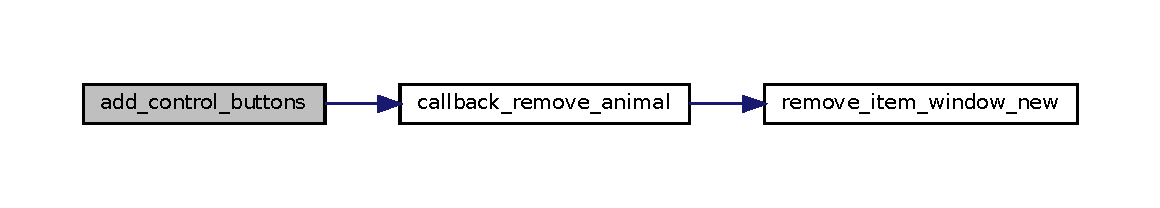
\includegraphics[width=350pt]{main__window_8h_acb8a7744ef425d1083a95017a3eaf1d7_cgraph}
\end{center}
\end{figure}
Here is the caller graph for this function\+:
\nopagebreak
\begin{figure}[H]
\begin{center}
\leavevmode
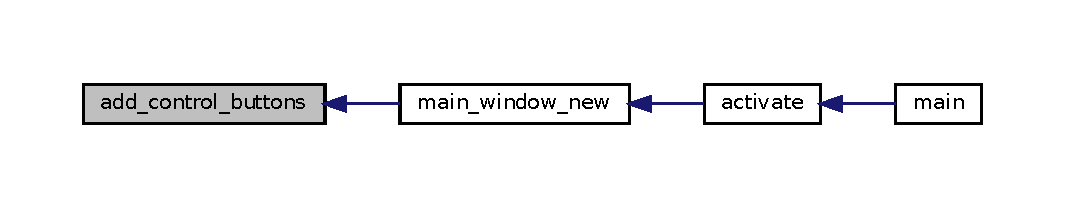
\includegraphics[width=350pt]{main__window_8h_acb8a7744ef425d1083a95017a3eaf1d7_icgraph}
\end{center}
\end{figure}
\mbox{\Hypertarget{main__window_8h_af1eaf0a9c2a7070f525386bb7ef4bac0}\label{main__window_8h_af1eaf0a9c2a7070f525386bb7ef4bac0}} 
\index{main\+\_\+window.\+h@{main\+\_\+window.\+h}!add\+\_\+table\+\_\+headers@{add\+\_\+table\+\_\+headers}}
\index{add\+\_\+table\+\_\+headers@{add\+\_\+table\+\_\+headers}!main\+\_\+window.\+h@{main\+\_\+window.\+h}}
\subsubsection{\texorpdfstring{add\+\_\+table\+\_\+headers()}{add\_table\_headers()}}
{\footnotesize\ttfamily void add\+\_\+table\+\_\+headers (\begin{DoxyParamCaption}\item[{Gtk\+Widget $\ast$}]{main\+Container,  }\item[{Gtk\+Widget $\ast$}]{table,  }\item[{\mbox{\hyperlink{struct_animal_linked_list}{Animal\+Linked\+List}} $\ast$}]{animals }\end{DoxyParamCaption})}



Add table header buttons. 


\begin{DoxyParams}{Parameters}
{\em main\+Container} & the main Gtk\+Grid of the window \\
\hline
{\em table} & table \\
\hline
{\em animals} & list of animals \\
\hline
\end{DoxyParams}


Definition at line 147 of file main\+\_\+window.\+c.



References A\+GE, callback\+\_\+sort\+\_\+click(), C\+O\+M\+M\+E\+NT, ID, N\+A\+ME, sort\+\_\+callback\+\_\+data\+\_\+new(), and S\+P\+E\+C\+I\+ES.



Referenced by main\+\_\+window\+\_\+new().


\begin{DoxyCode}
150 \{
151     GtkWidget *buttonId = gtk\_button\_new();
152     gtk\_button\_set\_label(GTK\_BUTTON(buttonId), \textcolor{stringliteral}{"Id"});
153     gtk\_widget\_set\_hexpand(buttonId, TRUE);
154 
155     g\_signal\_connect(G\_OBJECT(buttonId), \textcolor{stringliteral}{"clicked"}, G\_CALLBACK(
      \mbox{\hyperlink{main__window_8c_a14991586378d572e198ab90004e60e5d}{callback\_sort\_click}}), (gpointer) \mbox{\hyperlink{main__window_8c_a0d2178b065572d4806629a2efa02e1b8}{sort\_callback\_data\_new}}(
      \mbox{\hyperlink{main__window_8h_a727e9b9696032b380d0072840595ef05a001479a58fb44c39a29b20d565081a68}{ID}}, animals, table));
156     gtk\_grid\_attach(GTK\_GRID (mainContainer), GTK\_WIDGET (buttonId), 0, 0, 1, 1);
157 
158     GtkWidget *buttonName = gtk\_button\_new();
159     gtk\_button\_set\_label(GTK\_BUTTON(buttonName), \textcolor{stringliteral}{"Imię"});
160     gtk\_widget\_set\_hexpand(buttonName, TRUE);
161     g\_signal\_connect(G\_OBJECT(buttonName), \textcolor{stringliteral}{"clicked"}, G\_CALLBACK(
      \mbox{\hyperlink{main__window_8c_a14991586378d572e198ab90004e60e5d}{callback\_sort\_click}}), (gpointer) \mbox{\hyperlink{main__window_8c_a0d2178b065572d4806629a2efa02e1b8}{sort\_callback\_data\_new}}(
      \mbox{\hyperlink{main__window_8h_a727e9b9696032b380d0072840595ef05a67bc2ced260a8e43805d2480a785d312}{NAME}}, animals, table));
162     gtk\_widget\_set\_margin\_start(buttonName, 5);
163     gtk\_grid\_attach(GTK\_GRID (mainContainer), GTK\_WIDGET (buttonName), 1, 0, 1, 1);
164 
165     GtkWidget *buttonSpecies = gtk\_button\_new();
166     gtk\_button\_set\_label(GTK\_BUTTON(buttonSpecies), \textcolor{stringliteral}{"Gatunek"});
167     gtk\_widget\_set\_hexpand(buttonSpecies, TRUE);
168     g\_signal\_connect(G\_OBJECT(buttonSpecies), \textcolor{stringliteral}{"clicked"}, G\_CALLBACK(
      \mbox{\hyperlink{main__window_8c_a14991586378d572e198ab90004e60e5d}{callback\_sort\_click}}),
169                      (gpointer) \mbox{\hyperlink{main__window_8c_a0d2178b065572d4806629a2efa02e1b8}{sort\_callback\_data\_new}}(
      \mbox{\hyperlink{main__window_8h_a727e9b9696032b380d0072840595ef05a1663380252e067c51dd9ccc2b765691f}{SPECIES}}, animals, table));
170     gtk\_widget\_set\_margin\_start(buttonSpecies, 5);
171     gtk\_grid\_attach(GTK\_GRID (mainContainer), GTK\_WIDGET (buttonSpecies), 2, 0, 1, 1);
172 
173     GtkWidget* buttonAge = gtk\_button\_new();
174     gtk\_button\_set\_label(GTK\_BUTTON(buttonAge), \textcolor{stringliteral}{"Wiek"});
175     gtk\_widget\_set\_hexpand(buttonAge, TRUE);
176     g\_signal\_connect(G\_OBJECT(buttonAge), \textcolor{stringliteral}{"clicked"}, G\_CALLBACK(
      \mbox{\hyperlink{main__window_8c_a14991586378d572e198ab90004e60e5d}{callback\_sort\_click}}),
177                      (gpointer) \mbox{\hyperlink{main__window_8c_a0d2178b065572d4806629a2efa02e1b8}{sort\_callback\_data\_new}}(\mbox{\hyperlink{main__window_8h_a727e9b9696032b380d0072840595ef05a9fc6b2c465e5d1c9e839400fa1e1dfbc}{AGE}}, animals, table));
178     gtk\_widget\_set\_margin\_start(buttonAge, 5);
179     gtk\_grid\_attach(GTK\_GRID (mainContainer), GTK\_WIDGET (buttonAge), 3, 0, 1, 1);
180 
181     GtkWidget* buttonComment = gtk\_button\_new();
182     gtk\_button\_set\_label(GTK\_BUTTON(buttonComment), \textcolor{stringliteral}{"Komentarz"});
183     gtk\_widget\_set\_hexpand(buttonComment, TRUE);
184     g\_signal\_connect(G\_OBJECT(buttonComment), \textcolor{stringliteral}{"clicked"}, G\_CALLBACK(
      \mbox{\hyperlink{main__window_8c_a14991586378d572e198ab90004e60e5d}{callback\_sort\_click}}),
185                      (gpointer) \mbox{\hyperlink{main__window_8c_a0d2178b065572d4806629a2efa02e1b8}{sort\_callback\_data\_new}}(
      \mbox{\hyperlink{main__window_8h_a727e9b9696032b380d0072840595ef05aae696377c19e507b64e16be78ce3bbdb}{COMMENT}}, animals, table));
186     gtk\_widget\_set\_margin\_start(buttonComment, 5);
187     gtk\_grid\_attach(GTK\_GRID (mainContainer), GTK\_WIDGET (buttonComment), 4, 0, 1, 1);
188 \}
\end{DoxyCode}
Here is the call graph for this function\+:
\nopagebreak
\begin{figure}[H]
\begin{center}
\leavevmode
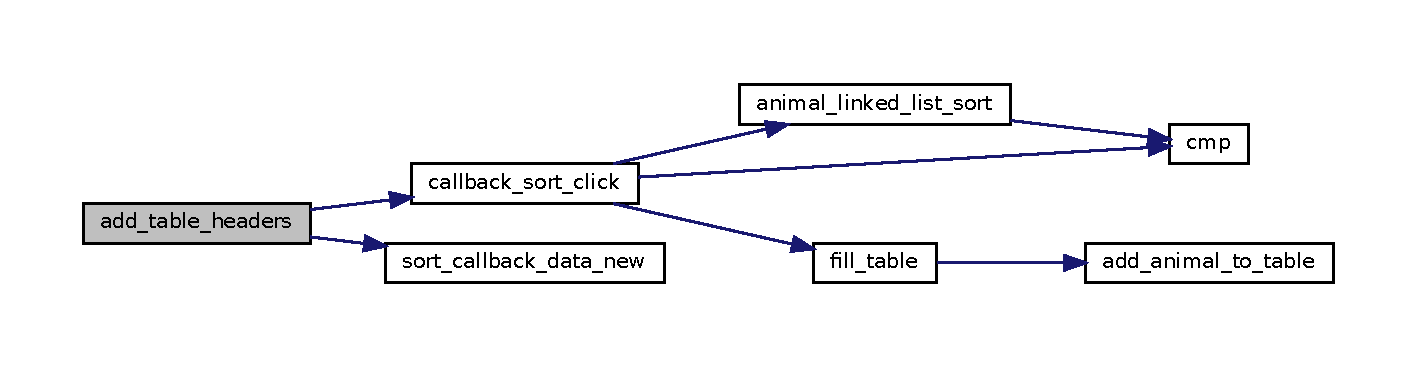
\includegraphics[width=350pt]{main__window_8h_af1eaf0a9c2a7070f525386bb7ef4bac0_cgraph}
\end{center}
\end{figure}
Here is the caller graph for this function\+:
\nopagebreak
\begin{figure}[H]
\begin{center}
\leavevmode
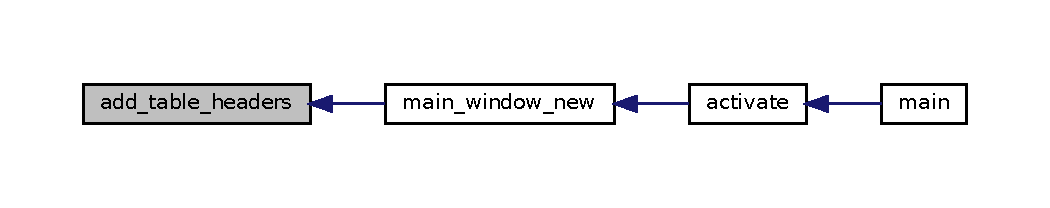
\includegraphics[width=350pt]{main__window_8h_af1eaf0a9c2a7070f525386bb7ef4bac0_icgraph}
\end{center}
\end{figure}
\mbox{\Hypertarget{main__window_8h_a14991586378d572e198ab90004e60e5d}\label{main__window_8h_a14991586378d572e198ab90004e60e5d}} 
\index{main\+\_\+window.\+h@{main\+\_\+window.\+h}!callback\+\_\+sort\+\_\+click@{callback\+\_\+sort\+\_\+click}}
\index{callback\+\_\+sort\+\_\+click@{callback\+\_\+sort\+\_\+click}!main\+\_\+window.\+h@{main\+\_\+window.\+h}}
\subsubsection{\texorpdfstring{callback\+\_\+sort\+\_\+click()}{callback\_sort\_click()}}
{\footnotesize\ttfamily void callback\+\_\+sort\+\_\+click (\begin{DoxyParamCaption}\item[{Gtk\+Widget $\ast$}]{widget,  }\item[{gpointer}]{callback\+\_\+data }\end{DoxyParamCaption})}

On click on any of the header buttons 
\begin{DoxyParams}{Parameters}
{\em widget} & \\
\hline
{\em callback\+\_\+data} & an instance of \mbox{\hyperlink{struct_sort_callback_data}{Sort\+Callback\+Data}} \\
\hline
\end{DoxyParams}


Definition at line 197 of file main\+\_\+window.\+c.



References animal\+\_\+linked\+\_\+list\+\_\+sort(), cmp(), Sort\+Callback\+Data\+::col, fill\+\_\+table(), Sort\+Callback\+Data\+::list, sort\+\_\+asc, sort\+\_\+by, and Sort\+Callback\+Data\+::table.



Referenced by add\+\_\+table\+\_\+headers().


\begin{DoxyCode}
200 \{
201     \mbox{\hyperlink{struct_sort_callback_data}{SortCallbackData}}* cd = (\mbox{\hyperlink{struct_sort_callback_data}{SortCallbackData}}*) callback\_data;
202     \textcolor{keywordflow}{if}(\mbox{\hyperlink{main__window_8c_ae80c4a7f36242f763719ea198dbec6b3}{sort\_by}} == cd->\mbox{\hyperlink{struct_sort_callback_data_a0e28c35278440f85596b96930dcf7025}{col}}) \mbox{\hyperlink{main__window_8c_abe63683d34822ebdd1f134edbfafb292}{sort\_asc}} = !\mbox{\hyperlink{main__window_8c_abe63683d34822ebdd1f134edbfafb292}{sort\_asc}};
203     \mbox{\hyperlink{main__window_8c_ae80c4a7f36242f763719ea198dbec6b3}{sort\_by}} = cd->\mbox{\hyperlink{struct_sort_callback_data_a0e28c35278440f85596b96930dcf7025}{col}};
204     \mbox{\hyperlink{animal_8h_a27f4c15c2d3176ea1ccea0b652f53a21}{animal\_linked\_list\_sort}}(cd->\mbox{\hyperlink{struct_sort_callback_data_a7fb8d190af45cd79bcf2f1cf986d018b}{list}}, \mbox{\hyperlink{main__window_8c_a2e261ff6f544c95d8ea3adab66a4252d}{cmp}});
205     \mbox{\hyperlink{main__window_8c_a7cd8ebd9f8b95eb48255fa9217843ca7}{fill\_table}}(cd->\mbox{\hyperlink{struct_sort_callback_data_a156725d482db7655e8817dc15865d191}{table}}, cd->\mbox{\hyperlink{struct_sort_callback_data_a7fb8d190af45cd79bcf2f1cf986d018b}{list}});
206 \}
\end{DoxyCode}
Here is the call graph for this function\+:
\nopagebreak
\begin{figure}[H]
\begin{center}
\leavevmode
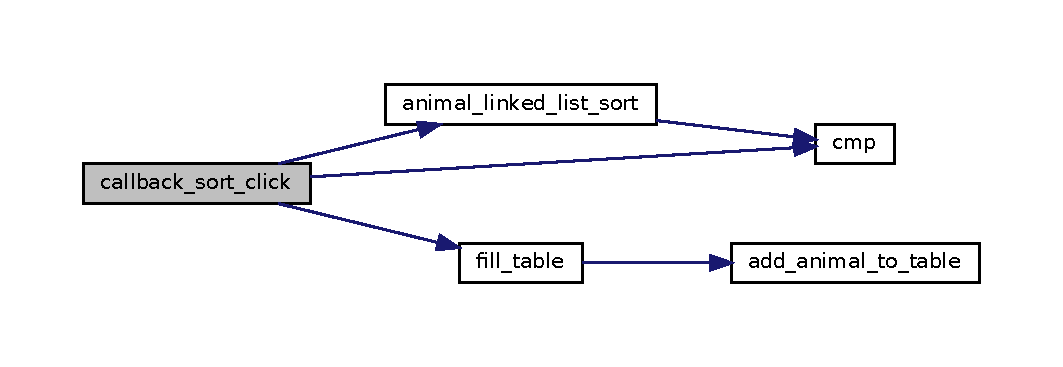
\includegraphics[width=350pt]{main__window_8h_a14991586378d572e198ab90004e60e5d_cgraph}
\end{center}
\end{figure}
Here is the caller graph for this function\+:
\nopagebreak
\begin{figure}[H]
\begin{center}
\leavevmode
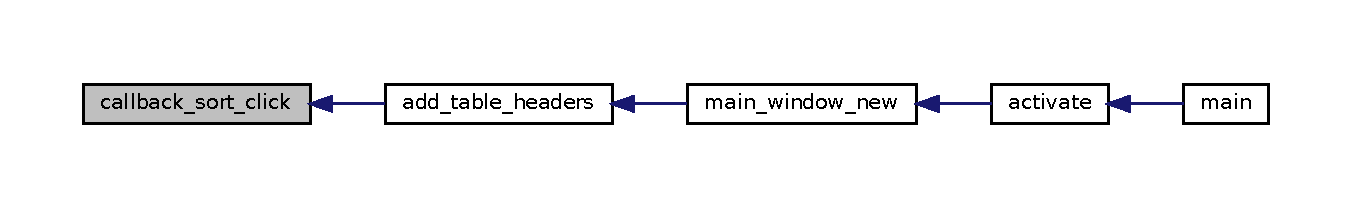
\includegraphics[width=350pt]{main__window_8h_a14991586378d572e198ab90004e60e5d_icgraph}
\end{center}
\end{figure}
\mbox{\Hypertarget{main__window_8h_a7cd8ebd9f8b95eb48255fa9217843ca7}\label{main__window_8h_a7cd8ebd9f8b95eb48255fa9217843ca7}} 
\index{main\+\_\+window.\+h@{main\+\_\+window.\+h}!fill\+\_\+table@{fill\+\_\+table}}
\index{fill\+\_\+table@{fill\+\_\+table}!main\+\_\+window.\+h@{main\+\_\+window.\+h}}
\subsubsection{\texorpdfstring{fill\+\_\+table()}{fill\_table()}}
{\footnotesize\ttfamily void fill\+\_\+table (\begin{DoxyParamCaption}\item[{Gtk\+Widget $\ast$}]{table,  }\item[{\mbox{\hyperlink{struct_animal_linked_list}{Animal\+Linked\+List}} $\ast$}]{animals }\end{DoxyParamCaption})}



Definition at line 264 of file main\+\_\+window.\+c.



References add\+\_\+animal\+\_\+to\+\_\+table(), Animal\+Linked\+List\+::first\+Item, Animal\+Linked\+List\+Item\+::next, Animal\+Linked\+List\+::size, and Animal\+Linked\+List\+Item\+::value.



Referenced by callback\+\_\+sort\+\_\+click(), and main\+\_\+window\+\_\+new().


\begin{DoxyCode}
266 \{
267     GList *children, *iter;
268 
269     children = gtk\_container\_get\_children(GTK\_CONTAINER(table));
270     \textcolor{keywordflow}{for}(iter = children; iter != NULL; iter = g\_list\_next(iter))
271         gtk\_widget\_destroy(GTK\_WIDGET(iter->data));
272     g\_list\_free(children);
273 
274     \mbox{\hyperlink{struct_animal_linked_list_item}{AnimalLinkedListItem}}* cur = animals->\mbox{\hyperlink{struct_animal_linked_list_a3a2756757903e7f1a69336bc78cc877a}{firstItem}};
275     \textcolor{keywordflow}{for}(\textcolor{keywordtype}{int} i=0; i<animals->\mbox{\hyperlink{struct_animal_linked_list_a28ace4cc471481a60e6a9bb41c9de892}{size}}; ++i)\{
276         \mbox{\hyperlink{main__window_8c_ab6218d4bd60fdaaf750c94cec25da675}{add\_animal\_to\_table}}(table, cur->\mbox{\hyperlink{struct_animal_linked_list_item_a6beaaaa5100f3f9f3cb09b5746208047}{value}}, i+1);
277         cur = cur->\mbox{\hyperlink{struct_animal_linked_list_item_a06cafc1028de611d48fcbe0ead6317ad}{next}};
278     \}
279 \}
\end{DoxyCode}
Here is the call graph for this function\+:
\nopagebreak
\begin{figure}[H]
\begin{center}
\leavevmode
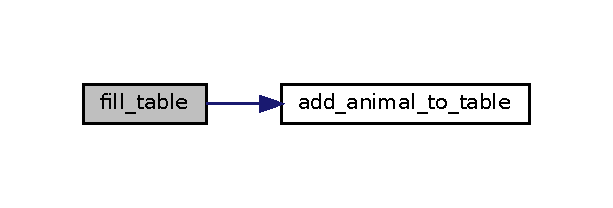
\includegraphics[width=294pt]{main__window_8h_a7cd8ebd9f8b95eb48255fa9217843ca7_cgraph}
\end{center}
\end{figure}
Here is the caller graph for this function\+:
\nopagebreak
\begin{figure}[H]
\begin{center}
\leavevmode
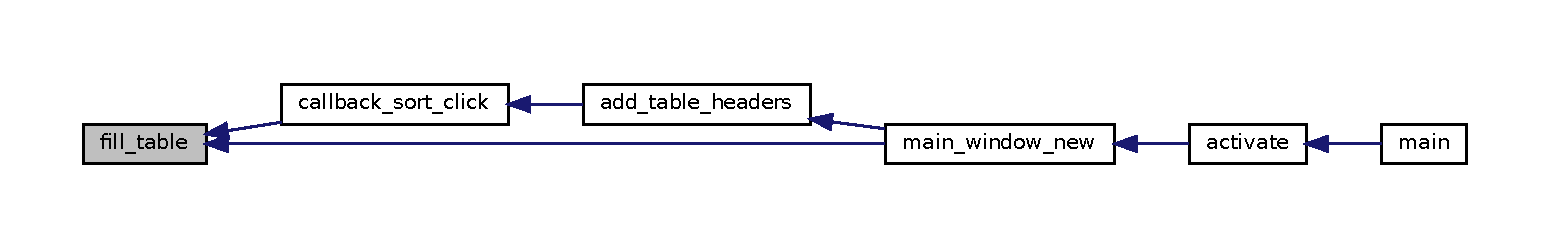
\includegraphics[width=350pt]{main__window_8h_a7cd8ebd9f8b95eb48255fa9217843ca7_icgraph}
\end{center}
\end{figure}
\mbox{\Hypertarget{main__window_8h_adcf0e83db47ee039761c9b42887a6c6c}\label{main__window_8h_adcf0e83db47ee039761c9b42887a6c6c}} 
\index{main\+\_\+window.\+h@{main\+\_\+window.\+h}!main\+\_\+window\+\_\+new@{main\+\_\+window\+\_\+new}}
\index{main\+\_\+window\+\_\+new@{main\+\_\+window\+\_\+new}!main\+\_\+window.\+h@{main\+\_\+window.\+h}}
\subsubsection{\texorpdfstring{main\+\_\+window\+\_\+new()}{main\_window\_new()}}
{\footnotesize\ttfamily Gtk\+Widget$\ast$ main\+\_\+window\+\_\+new (\begin{DoxyParamCaption}\item[{Gtk\+Application $\ast$}]{app }\end{DoxyParamCaption})}



Initialize the main window. 


\begin{DoxyParams}{Parameters}
{\em app} & Application \\
\hline
\end{DoxyParams}
\begin{DoxyReturn}{Returns}
main window, not shown yet 
\end{DoxyReturn}


Definition at line 49 of file main\+\_\+window.\+c.



References add\+\_\+control\+\_\+buttons(), add\+\_\+table\+\_\+headers(), animal\+\_\+linked\+\_\+list\+\_\+add\+\_\+item(), animal\+\_\+linked\+\_\+list\+\_\+new(), animal\+\_\+new(), and fill\+\_\+table().



Referenced by activate().


\begin{DoxyCode}
50 \{
51 
52     GtkWidget* window;
53     GtkWidget* mainContainer;
54 
55     window = gtk\_application\_window\_new (app);
56     gtk\_window\_set\_title (GTK\_WINDOW (window), \textcolor{stringliteral}{"Ogród zoologiczny"});
57     gtk\_window\_set\_default\_size (GTK\_WINDOW (window), 500, 500);
58 
59     mainContainer = gtk\_grid\_new();
60     gtk\_container\_add(GTK\_CONTAINER (window), GTK\_WIDGET (mainContainer));
61 
62     GtkWidget* containerTable;
63     containerTable = gtk\_scrolled\_window\_new(NULL, NULL);
64     gtk\_widget\_set\_hexpand(containerTable, 1);
65     gtk\_widget\_set\_vexpand(containerTable, 1);
66     GtkWidget* table;
67     table = gtk\_grid\_new();
68     \mbox{\hyperlink{struct_animal_linked_list}{AnimalLinkedList}}* animals = \mbox{\hyperlink{animal_8h_a5d57c899f6584a225dda3cacc771a1b7}{animal\_linked\_list\_new}}();
69 
70     \textcolor{keywordflow}{for}(\textcolor{keywordtype}{int} i=0; i<200; ++i)\{
71         \mbox{\hyperlink{struct_animal}{Animal}}* a = \mbox{\hyperlink{animal_8h_af6d6189ffd7e3fb411e0c2e7386b5103}{animal\_new}}(i, \textcolor{stringliteral}{"Blazej"}, \textcolor{stringliteral}{"Wielblad"}, i/4+3, \textcolor{stringliteral}{"Je orzeszki"});
72         \mbox{\hyperlink{animal_8h_a56aa81831577f1bc41977c699e832363}{animal\_linked\_list\_add\_item}}(animals, a);
73     \}
74     gtk\_container\_add(GTK\_CONTAINER(containerTable), GTK\_WIDGET(table));
75     gtk\_grid\_set\_column\_homogeneous(GTK\_GRID(table), gtk\_true());
76     gtk\_grid\_set\_column\_homogeneous(GTK\_GRID(mainContainer), gtk\_true());
77     \mbox{\hyperlink{main__window_8c_af1eaf0a9c2a7070f525386bb7ef4bac0}{add\_table\_headers}}(mainContainer, table, animals);
78     \mbox{\hyperlink{main__window_8c_a7cd8ebd9f8b95eb48255fa9217843ca7}{fill\_table}}(table, animals);
79     gtk\_grid\_attach(GTK\_GRID (mainContainer), GTK\_WIDGET (containerTable), 0, 1, 5, 1);
80     \mbox{\hyperlink{main__window_8c_acb8a7744ef425d1083a95017a3eaf1d7}{add\_control\_buttons}}(app, mainContainer);
81 
82     \textcolor{keywordflow}{return} window;
83 \}
\end{DoxyCode}
Here is the call graph for this function\+:
\nopagebreak
\begin{figure}[H]
\begin{center}
\leavevmode
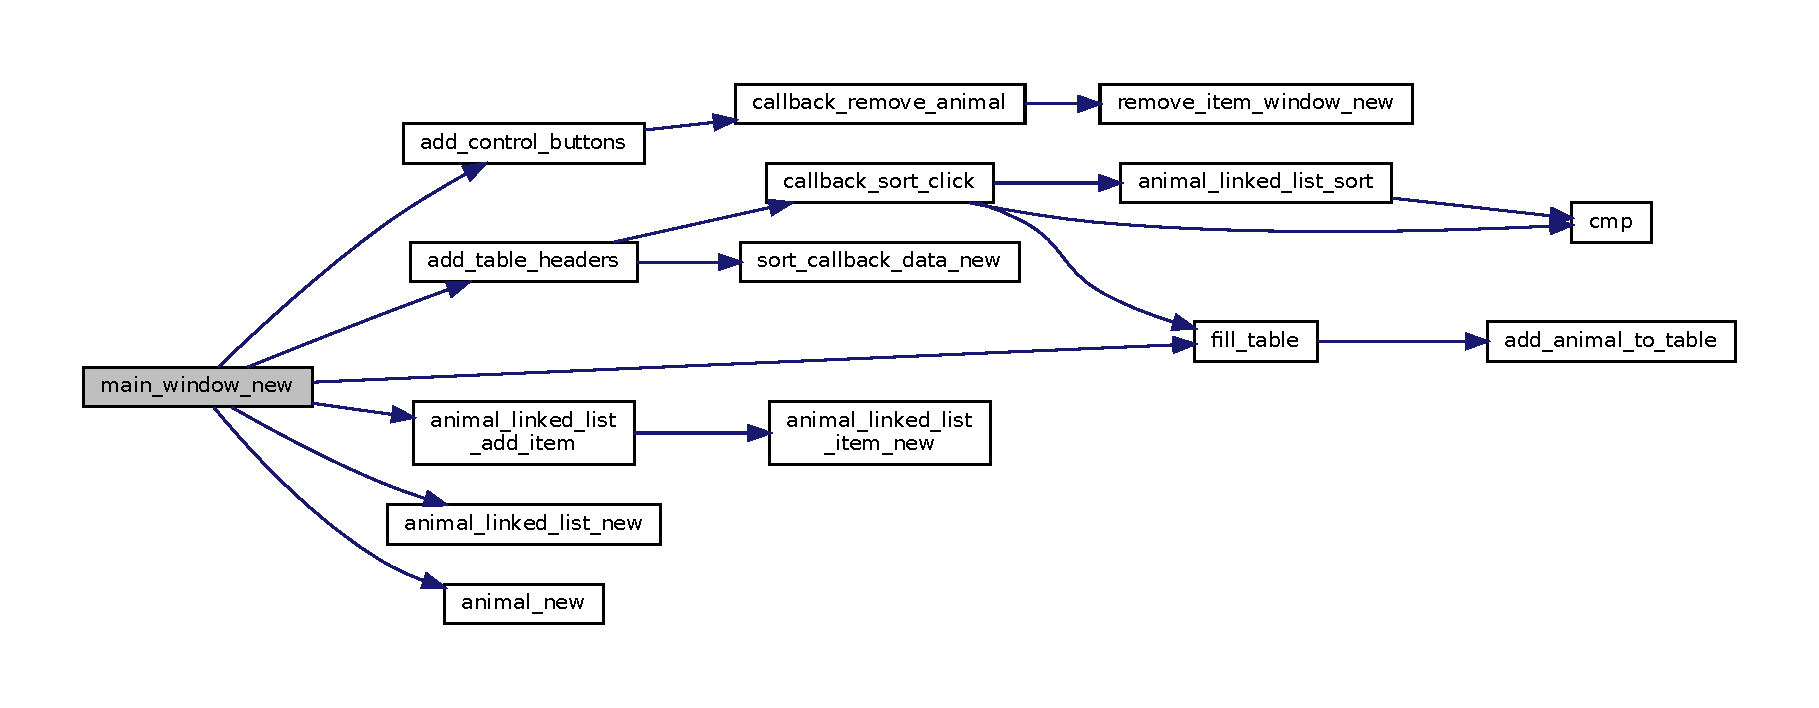
\includegraphics[width=350pt]{main__window_8h_adcf0e83db47ee039761c9b42887a6c6c_cgraph}
\end{center}
\end{figure}
Here is the caller graph for this function\+:
\nopagebreak
\begin{figure}[H]
\begin{center}
\leavevmode
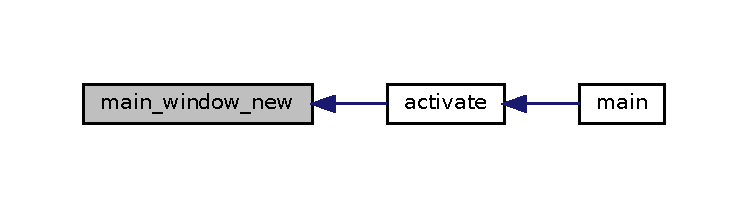
\includegraphics[width=350pt]{main__window_8h_adcf0e83db47ee039761c9b42887a6c6c_icgraph}
\end{center}
\end{figure}

\hypertarget{http_8h}{}\section{include/services/http.h File Reference}
\label{http_8h}\index{include/services/http.\+h@{include/services/http.\+h}}
This graph shows which files directly or indirectly include this file\+:
\nopagebreak
\begin{figure}[H]
\begin{center}
\leavevmode
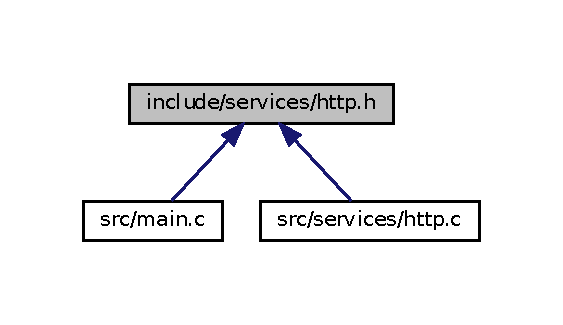
\includegraphics[width=270pt]{http_8h__dep__incl}
\end{center}
\end{figure}
\subsection*{Data Structures}
\begin{DoxyCompactItemize}
\item 
struct \mbox{\hyperlink{struct_http_response}{Http\+Response}}
\end{DoxyCompactItemize}
\subsection*{Typedefs}
\begin{DoxyCompactItemize}
\item 
typedef struct \mbox{\hyperlink{struct_http_response}{Http\+Response}} \mbox{\hyperlink{http_8h_a759eca53484c77acda459c191b9efa1f}{Http\+Response}}
\end{DoxyCompactItemize}
\subsection*{Functions}
\begin{DoxyCompactItemize}
\item 
size\+\_\+t \mbox{\hyperlink{http_8h_a4c00439adfc2c266dfc3f138a4bab5bb}{write\+\_\+function}} (void $\ast$ptr, size\+\_\+t size, size\+\_\+t nmemb, \mbox{\hyperlink{struct_http_response}{Http\+Response}} $\ast$r)
\item 
\mbox{\hyperlink{struct_http_response}{Http\+Response}} $\ast$ \mbox{\hyperlink{http_8h_a38c946ac3ac1ac192d43cb6595fdf5c3}{http\+\_\+get}} (char $\ast$url)
\begin{DoxyCompactList}\small\item\em Gets H\+T\+TP response for url. \end{DoxyCompactList}\end{DoxyCompactItemize}


\subsection{Typedef Documentation}
\mbox{\Hypertarget{http_8h_a759eca53484c77acda459c191b9efa1f}\label{http_8h_a759eca53484c77acda459c191b9efa1f}} 
\index{http.\+h@{http.\+h}!Http\+Response@{Http\+Response}}
\index{Http\+Response@{Http\+Response}!http.\+h@{http.\+h}}
\subsubsection{\texorpdfstring{Http\+Response}{HttpResponse}}
{\footnotesize\ttfamily typedef struct \mbox{\hyperlink{struct_http_response}{Http\+Response}}  \mbox{\hyperlink{struct_http_response}{Http\+Response}}}



\subsection{Function Documentation}
\mbox{\Hypertarget{http_8h_a38c946ac3ac1ac192d43cb6595fdf5c3}\label{http_8h_a38c946ac3ac1ac192d43cb6595fdf5c3}} 
\index{http.\+h@{http.\+h}!http\+\_\+get@{http\+\_\+get}}
\index{http\+\_\+get@{http\+\_\+get}!http.\+h@{http.\+h}}
\subsubsection{\texorpdfstring{http\+\_\+get()}{http\_get()}}
{\footnotesize\ttfamily \mbox{\hyperlink{struct_http_response}{Http\+Response}}$\ast$ http\+\_\+get (\begin{DoxyParamCaption}\item[{char $\ast$}]{url }\end{DoxyParamCaption})}



Gets H\+T\+TP response for url. 


\begin{DoxyParams}{Parameters}
{\em url} & Site address \\
\hline
\end{DoxyParams}
\begin{DoxyReturn}{Returns}
Filled \mbox{\hyperlink{struct_http_response}{Http\+Response}} 
\end{DoxyReturn}


Definition at line 33 of file http.\+c.



References Http\+Response\+::code, Http\+Response\+::data, http\+\_\+response\+\_\+new(), and write\+\_\+function().



Referenced by main().


\begin{DoxyCode}
33                                    \{
34     CURL *curl;
35     \mbox{\hyperlink{struct_http_response}{HttpResponse}} * res = \mbox{\hyperlink{http_8c_a47626df99e751c22b12fc185e4d84d7d}{http\_response\_new}}();
36 
37     curl = curl\_easy\_init();
38     \textcolor{keywordflow}{if}(curl) \{
39         puts(url);
40         curl\_easy\_setopt(curl, CURLOPT\_URL, url);
41         \textcolor{comment}{/* example.com is redirected, so we tell libcurl to follow redirection */}
42         curl\_easy\_setopt(curl, CURLOPT\_FOLLOWLOCATION, 1L);
43         curl\_easy\_setopt(curl, CURLOPT\_WRITEFUNCTION, \mbox{\hyperlink{http_8c_a4c00439adfc2c266dfc3f138a4bab5bb}{write\_function}});
44         curl\_easy\_setopt(curl, CURLOPT\_WRITEDATA, res);
45 
46         \textcolor{comment}{/* Perform the request, res will get the return code */}
47         res->\mbox{\hyperlink{struct_http_response_abce68ae6776a536dce762f0b6a96ab54}{code}} = curl\_easy\_perform(curl);
48         \textcolor{comment}{/* Check for errors */}
49         \textcolor{keywordflow}{if}(res->\mbox{\hyperlink{struct_http_response_abce68ae6776a536dce762f0b6a96ab54}{code}} != CURLE\_OK)
50             fprintf(stderr, \textcolor{stringliteral}{"curl\_easy\_perform() failed: %s\(\backslash\)n"},
51                     curl\_easy\_strerror(res->\mbox{\hyperlink{struct_http_response_abce68ae6776a536dce762f0b6a96ab54}{code}}));
52         \textcolor{keywordflow}{else} \{
53             printf(\textcolor{stringliteral}{"Data: %s\(\backslash\)n"}, res->\mbox{\hyperlink{struct_http_response_a29b7ecfb11da1af6c7fdd3fe7862901f}{data}});
54         \}
55 
56         \textcolor{comment}{/* always cleanup */}
57         curl\_easy\_cleanup(curl);
58     \}
59     \textcolor{keywordflow}{return} res;
60 \}
\end{DoxyCode}
Here is the call graph for this function\+:
\nopagebreak
\begin{figure}[H]
\begin{center}
\leavevmode
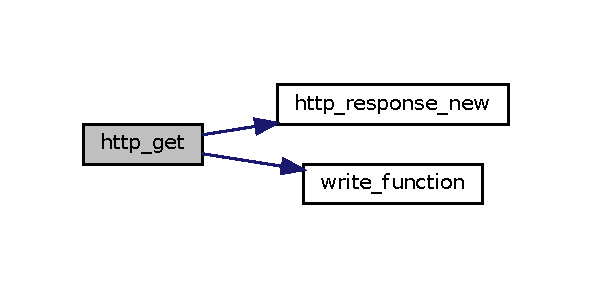
\includegraphics[width=284pt]{http_8h_a38c946ac3ac1ac192d43cb6595fdf5c3_cgraph}
\end{center}
\end{figure}
Here is the caller graph for this function\+:
\nopagebreak
\begin{figure}[H]
\begin{center}
\leavevmode
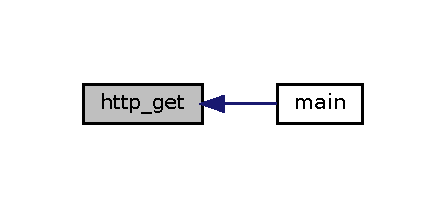
\includegraphics[width=214pt]{http_8h_a38c946ac3ac1ac192d43cb6595fdf5c3_icgraph}
\end{center}
\end{figure}
\mbox{\Hypertarget{http_8h_a4c00439adfc2c266dfc3f138a4bab5bb}\label{http_8h_a4c00439adfc2c266dfc3f138a4bab5bb}} 
\index{http.\+h@{http.\+h}!write\+\_\+function@{write\+\_\+function}}
\index{write\+\_\+function@{write\+\_\+function}!http.\+h@{http.\+h}}
\subsubsection{\texorpdfstring{write\+\_\+function()}{write\_function()}}
{\footnotesize\ttfamily size\+\_\+t write\+\_\+function (\begin{DoxyParamCaption}\item[{void $\ast$}]{ptr,  }\item[{size\+\_\+t}]{size,  }\item[{size\+\_\+t}]{nmemb,  }\item[{\mbox{\hyperlink{struct_http_response}{Http\+Response}} $\ast$}]{r }\end{DoxyParamCaption})}



Definition at line 12 of file http.\+c.



References Http\+Response\+::data, and Http\+Response\+::size.



Referenced by http\+\_\+get().


\begin{DoxyCode}
12                                                                             \{
13     \textcolor{keywordtype}{size\_t} new\_len = r->\mbox{\hyperlink{struct_http_response_a11b910682b365528a15fcfd6d4dd824f}{size}} + size*nmemb;
14     r->\mbox{\hyperlink{struct_http_response_a29b7ecfb11da1af6c7fdd3fe7862901f}{data}}= realloc(r->\mbox{\hyperlink{struct_http_response_a29b7ecfb11da1af6c7fdd3fe7862901f}{data}}, new\_len+1);
15     memcpy(r->\mbox{\hyperlink{struct_http_response_a29b7ecfb11da1af6c7fdd3fe7862901f}{data}}+r->\mbox{\hyperlink{struct_http_response_a11b910682b365528a15fcfd6d4dd824f}{size}}, ptr, size*nmemb);
16     r->\mbox{\hyperlink{struct_http_response_a29b7ecfb11da1af6c7fdd3fe7862901f}{data}}[new\_len] = \textcolor{charliteral}{'\(\backslash\)0'};
17     \textcolor{keywordflow}{return} size*nmemb;
18 \}
\end{DoxyCode}
Here is the caller graph for this function\+:
\nopagebreak
\begin{figure}[H]
\begin{center}
\leavevmode
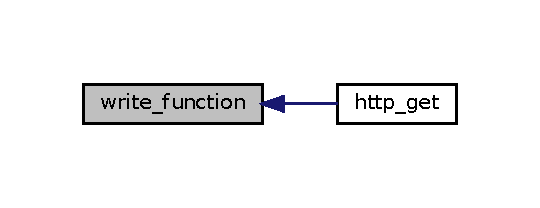
\includegraphics[width=336pt]{http_8h_a4c00439adfc2c266dfc3f138a4bab5bb_icgraph}
\end{center}
\end{figure}

\hypertarget{main_8c}{}\section{src/main.c File Reference}
\label{main_8c}\index{src/main.\+c@{src/main.\+c}}
{\ttfamily \#include $<$gtk/gtk.\+h$>$}\newline
{\ttfamily \#include $<$curl/curl.\+h$>$}\newline
{\ttfamily \#include \char`\"{}../include/main\+\_\+window.\+h\char`\"{}}\newline
{\ttfamily \#include \char`\"{}../include/services/http.\+h\char`\"{}}\newline
Include dependency graph for main.\+c\+:
\nopagebreak
\begin{figure}[H]
\begin{center}
\leavevmode
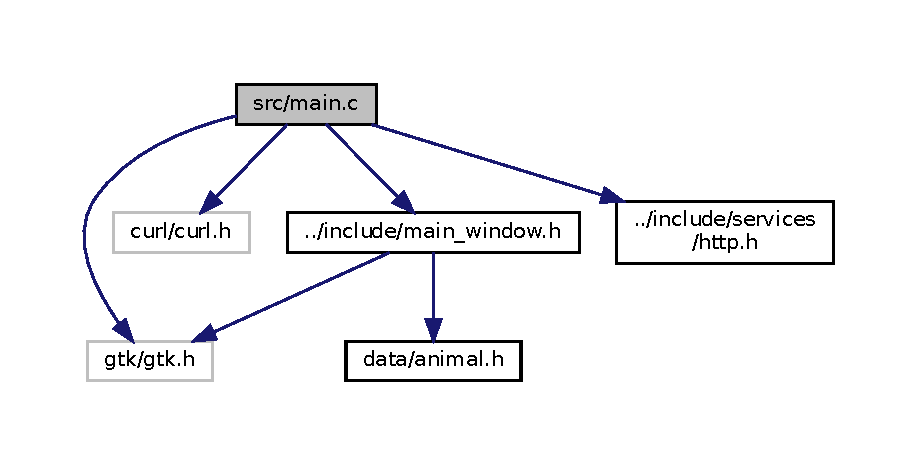
\includegraphics[width=350pt]{main_8c__incl}
\end{center}
\end{figure}
\subsection*{Functions}
\begin{DoxyCompactItemize}
\item 
static void \mbox{\hyperlink{main_8c_ac8d185b1db8b0153f14fd5cb4537cf2a}{activate}} (Gtk\+Application $\ast$app, gpointer user\+\_\+data)
\begin{DoxyCompactList}\small\item\em Initialize UI. \end{DoxyCompactList}\item 
int \mbox{\hyperlink{main_8c_a3c04138a5bfe5d72780bb7e82a18e627}{main}} (int argc, char $\ast$$\ast$argv)
\end{DoxyCompactItemize}


\subsection{Function Documentation}
\mbox{\Hypertarget{main_8c_ac8d185b1db8b0153f14fd5cb4537cf2a}\label{main_8c_ac8d185b1db8b0153f14fd5cb4537cf2a}} 
\index{main.\+c@{main.\+c}!activate@{activate}}
\index{activate@{activate}!main.\+c@{main.\+c}}
\subsubsection{\texorpdfstring{activate()}{activate()}}
{\footnotesize\ttfamily static void activate (\begin{DoxyParamCaption}\item[{Gtk\+Application $\ast$}]{app,  }\item[{gpointer}]{user\+\_\+data }\end{DoxyParamCaption})\hspace{0.3cm}{\ttfamily [static]}}



Initialize UI. 



Definition at line 10 of file main.\+c.



References main\+\_\+window\+\_\+new().



Referenced by main().


\begin{DoxyCode}
11 \{
12     \mbox{\hyperlink{main__window_8h_adcf0e83db47ee039761c9b42887a6c6c}{main\_window\_new}}(app);
13 \}
\end{DoxyCode}
Here is the call graph for this function\+:
\nopagebreak
\begin{figure}[H]
\begin{center}
\leavevmode
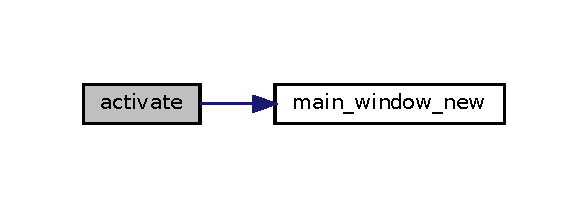
\includegraphics[width=282pt]{main_8c_ac8d185b1db8b0153f14fd5cb4537cf2a_cgraph}
\end{center}
\end{figure}
Here is the caller graph for this function\+:
\nopagebreak
\begin{figure}[H]
\begin{center}
\leavevmode
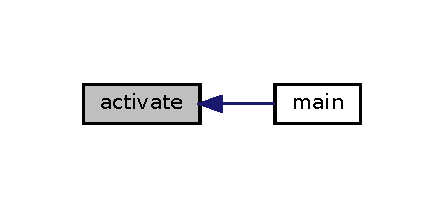
\includegraphics[width=213pt]{main_8c_ac8d185b1db8b0153f14fd5cb4537cf2a_icgraph}
\end{center}
\end{figure}
\mbox{\Hypertarget{main_8c_a3c04138a5bfe5d72780bb7e82a18e627}\label{main_8c_a3c04138a5bfe5d72780bb7e82a18e627}} 
\index{main.\+c@{main.\+c}!main@{main}}
\index{main@{main}!main.\+c@{main.\+c}}
\subsubsection{\texorpdfstring{main()}{main()}}
{\footnotesize\ttfamily int main (\begin{DoxyParamCaption}\item[{int}]{argc,  }\item[{char $\ast$$\ast$}]{argv }\end{DoxyParamCaption})}



Definition at line 15 of file main.\+c.



References activate(), and http\+\_\+get().


\begin{DoxyCode}
15                                \{
16     GtkApplication *app;
17 
18     \mbox{\hyperlink{http_8h_a38c946ac3ac1ac192d43cb6595fdf5c3}{http\_get}}(\textcolor{stringliteral}{"https://mrokita.pl/"});
19     \textcolor{keywordtype}{int} status;
20     app = gtk\_application\_new (\textcolor{stringliteral}{"pl.mrokita.pri3"}, G\_APPLICATION\_FLAGS\_NONE);
21     g\_signal\_connect (app, \textcolor{stringliteral}{"activate"}, G\_CALLBACK (\mbox{\hyperlink{main_8c_ac8d185b1db8b0153f14fd5cb4537cf2a}{activate}}), NULL);
22     status = g\_application\_run (G\_APPLICATION (app), argc, argv);
23     g\_object\_unref (app);
24 
25     \textcolor{keywordflow}{return} status;
26 \}
\end{DoxyCode}
Here is the call graph for this function\+:
\nopagebreak
\begin{figure}[H]
\begin{center}
\leavevmode
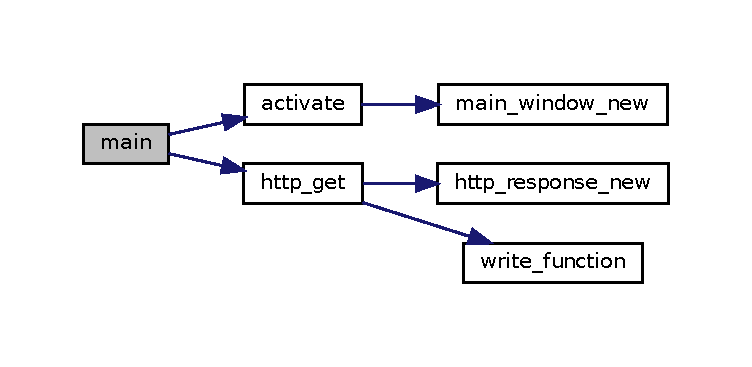
\includegraphics[width=350pt]{main_8c_a3c04138a5bfe5d72780bb7e82a18e627_cgraph}
\end{center}
\end{figure}

\hypertarget{main__window_8c}{}\section{src/main\+\_\+window.c File Reference}
\label{main__window_8c}\index{src/main\+\_\+window.\+c@{src/main\+\_\+window.\+c}}
{\ttfamily \#include \char`\"{}../include/main\+\_\+window.\+h\char`\"{}}\newline
Include dependency graph for main\+\_\+window.\+c\+:
\nopagebreak
\begin{figure}[H]
\begin{center}
\leavevmode
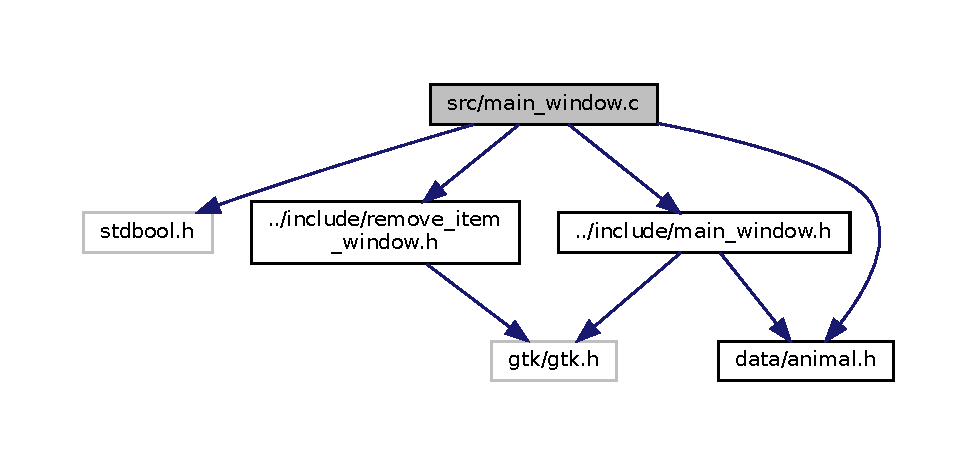
\includegraphics[width=220pt]{main__window_8c__incl}
\end{center}
\end{figure}
\subsection*{Functions}
\begin{DoxyCompactItemize}
\item 
Gtk\+Widget $\ast$ \mbox{\hyperlink{main__window_8c_adcf0e83db47ee039761c9b42887a6c6c}{main\+\_\+window\+\_\+new}} (Gtk\+Application $\ast$app)
\end{DoxyCompactItemize}


\subsection{Function Documentation}
\mbox{\Hypertarget{main__window_8c_adcf0e83db47ee039761c9b42887a6c6c}\label{main__window_8c_adcf0e83db47ee039761c9b42887a6c6c}} 
\index{main\+\_\+window.\+c@{main\+\_\+window.\+c}!main\+\_\+window\+\_\+new@{main\+\_\+window\+\_\+new}}
\index{main\+\_\+window\+\_\+new@{main\+\_\+window\+\_\+new}!main\+\_\+window.\+c@{main\+\_\+window.\+c}}
\subsubsection{\texorpdfstring{main\+\_\+window\+\_\+new()}{main\_window\_new()}}
{\footnotesize\ttfamily Gtk\+Widget$\ast$ main\+\_\+window\+\_\+new (\begin{DoxyParamCaption}\item[{Gtk\+Application $\ast$}]{app }\end{DoxyParamCaption})}



Definition at line 7 of file main\+\_\+window.\+c.



Referenced by activate().


\begin{DoxyCode}
7                                                 \{
8     GtkWidget *window;
9     GtkWidget *mainContainer;
10 
11     window = gtk\_application\_window\_new (app);
12     gtk\_window\_set\_title (GTK\_WINDOW (window), \textcolor{stringliteral}{"Ogród zoologiczny"});
13     gtk\_window\_set\_default\_size (GTK\_WINDOW (window), 500, 500);
14 
15     mainContainer = gtk\_grid\_new();
16     gtk\_container\_add(GTK\_CONTAINER (window), GTK\_WIDGET (mainContainer));
17 
18     GtkWidget *containerTable;
19     containerTable = gtk\_scrolled\_window\_new(NULL, NULL);
20     gtk\_widget\_set\_hexpand(containerTable, 1);
21     gtk\_widget\_set\_vexpand(containerTable, 1);
22     GtkWidget *table;
23     table = gtk\_grid\_new();
24     gtk\_container\_add(GTK\_CONTAINER(containerTable), GTK\_WIDGET(table));
25     \textcolor{keywordflow}{for}(\textcolor{keywordtype}{int} i=0; i<200; ++i)\{
26         GtkWidget *label = gtk\_label\_new(\textcolor{stringliteral}{"Test"});
27         gtk\_label\_set\_xalign(GTK\_LABEL (label), 0.0);
28         gtk\_widget\_set\_margin\_start(label, 5);
29         gtk\_widget\_set\_margin\_top(label, 5);
30         gtk\_widget\_set\_hexpand(label, TRUE);
31         gtk\_grid\_attach(GTK\_GRID (table), label, 0, i, 1, 1);
32     \}
33 
34     gtk\_grid\_attach(GTK\_GRID (mainContainer), GTK\_WIDGET (containerTable), 0, 1, 1, 1);
35 
36     GtkWidget *buttonAddAnimal;
37     buttonAddAnimal = gtk\_button\_new();
38     gtk\_button\_set\_label(GTK\_BUTTON (buttonAddAnimal), \textcolor{stringliteral}{"Dodaj zwierzę"});
39     gtk\_grid\_attach(GTK\_GRID (mainContainer), GTK\_WIDGET (buttonAddAnimal), 0, 2, 1, 1);
40     gtk\_widget\_set\_hexpand(buttonAddAnimal, 1);
41     gtk\_widget\_show\_all (window);
42 \}
\end{DoxyCode}
Here is the caller graph for this function\+:
\nopagebreak
\begin{figure}[H]
\begin{center}
\leavevmode
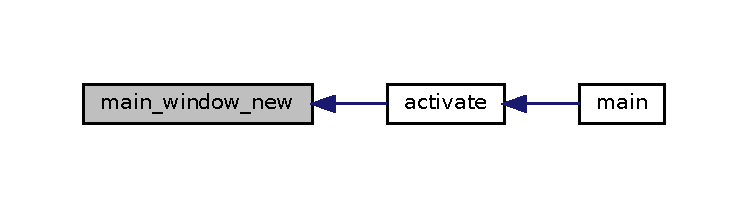
\includegraphics[width=350pt]{main__window_8c_adcf0e83db47ee039761c9b42887a6c6c_icgraph}
\end{center}
\end{figure}

\hypertarget{http_8c}{}\section{src/services/http.c File Reference}
\label{http_8c}\index{src/services/http.\+c@{src/services/http.\+c}}
{\ttfamily \#include $<$curl/curl.\+h$>$}\newline
{\ttfamily \#include $<$stdlib.\+h$>$}\newline
{\ttfamily \#include $<$string.\+h$>$}\newline
{\ttfamily \#include $<$stdio.\+h$>$}\newline
{\ttfamily \#include \char`\"{}../../include/services/http.\+h\char`\"{}}\newline
Include dependency graph for http.\+c\+:
\nopagebreak
\begin{figure}[H]
\begin{center}
\leavevmode
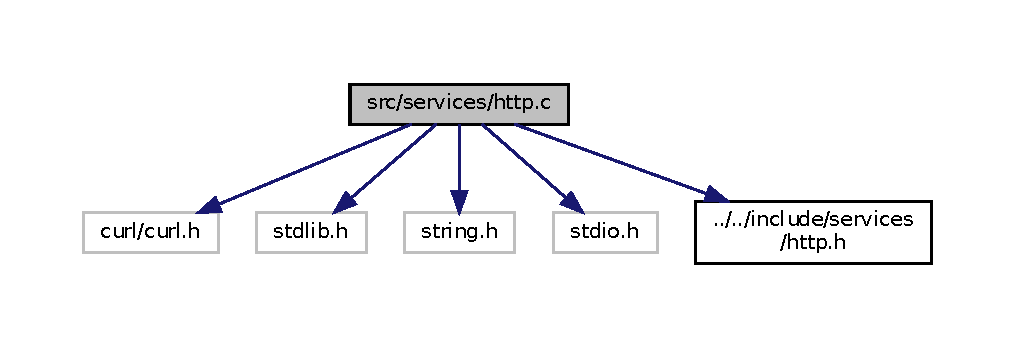
\includegraphics[width=350pt]{http_8c__incl}
\end{center}
\end{figure}
\subsection*{Functions}
\begin{DoxyCompactItemize}
\item 
size\+\_\+t \mbox{\hyperlink{http_8c_a4c00439adfc2c266dfc3f138a4bab5bb}{write\+\_\+function}} (void $\ast$ptr, size\+\_\+t size, size\+\_\+t nmemb, \mbox{\hyperlink{struct_http_response}{Http\+Response}} $\ast$r)
\item 
\mbox{\hyperlink{struct_http_response}{Http\+Response}} $\ast$ \mbox{\hyperlink{http_8c_a47626df99e751c22b12fc185e4d84d7d}{http\+\_\+response\+\_\+new}} ()
\item 
\mbox{\hyperlink{struct_http_response}{Http\+Response}} $\ast$ \mbox{\hyperlink{http_8c_a38c946ac3ac1ac192d43cb6595fdf5c3}{http\+\_\+get}} (char $\ast$url)
\begin{DoxyCompactList}\small\item\em Gets H\+T\+TP response for url. \end{DoxyCompactList}\end{DoxyCompactItemize}


\subsection{Function Documentation}
\mbox{\Hypertarget{http_8c_a38c946ac3ac1ac192d43cb6595fdf5c3}\label{http_8c_a38c946ac3ac1ac192d43cb6595fdf5c3}} 
\index{http.\+c@{http.\+c}!http\+\_\+get@{http\+\_\+get}}
\index{http\+\_\+get@{http\+\_\+get}!http.\+c@{http.\+c}}
\subsubsection{\texorpdfstring{http\+\_\+get()}{http\_get()}}
{\footnotesize\ttfamily \mbox{\hyperlink{struct_http_response}{Http\+Response}}$\ast$ http\+\_\+get (\begin{DoxyParamCaption}\item[{char $\ast$}]{url }\end{DoxyParamCaption})}



Gets H\+T\+TP response for url. 


\begin{DoxyParams}{Parameters}
{\em url} & Site address \\
\hline
\end{DoxyParams}
\begin{DoxyReturn}{Returns}
Filled \mbox{\hyperlink{struct_http_response}{Http\+Response}} 
\end{DoxyReturn}


Definition at line 33 of file http.\+c.



References Http\+Response\+::code, Http\+Response\+::data, http\+\_\+response\+\_\+new(), and write\+\_\+function().



Referenced by main().


\begin{DoxyCode}
33                                    \{
34     CURL *curl;
35     \mbox{\hyperlink{struct_http_response}{HttpResponse}} * res = \mbox{\hyperlink{http_8c_a47626df99e751c22b12fc185e4d84d7d}{http\_response\_new}}();
36 
37     curl = curl\_easy\_init();
38     \textcolor{keywordflow}{if}(curl) \{
39         puts(url);
40         curl\_easy\_setopt(curl, CURLOPT\_URL, url);
41         \textcolor{comment}{/* example.com is redirected, so we tell libcurl to follow redirection */}
42         curl\_easy\_setopt(curl, CURLOPT\_FOLLOWLOCATION, 1L);
43         curl\_easy\_setopt(curl, CURLOPT\_WRITEFUNCTION, \mbox{\hyperlink{http_8c_a4c00439adfc2c266dfc3f138a4bab5bb}{write\_function}});
44         curl\_easy\_setopt(curl, CURLOPT\_WRITEDATA, res);
45 
46         \textcolor{comment}{/* Perform the request, res will get the return code */}
47         res->\mbox{\hyperlink{struct_http_response_abce68ae6776a536dce762f0b6a96ab54}{code}} = curl\_easy\_perform(curl);
48         \textcolor{comment}{/* Check for errors */}
49         \textcolor{keywordflow}{if}(res->\mbox{\hyperlink{struct_http_response_abce68ae6776a536dce762f0b6a96ab54}{code}} != CURLE\_OK)
50             fprintf(stderr, \textcolor{stringliteral}{"curl\_easy\_perform() failed: %s\(\backslash\)n"},
51                     curl\_easy\_strerror(res->\mbox{\hyperlink{struct_http_response_abce68ae6776a536dce762f0b6a96ab54}{code}}));
52         \textcolor{keywordflow}{else} \{
53             printf(\textcolor{stringliteral}{"Data: %s\(\backslash\)n"}, res->\mbox{\hyperlink{struct_http_response_a29b7ecfb11da1af6c7fdd3fe7862901f}{data}});
54         \}
55 
56         \textcolor{comment}{/* always cleanup */}
57         curl\_easy\_cleanup(curl);
58     \}
59     \textcolor{keywordflow}{return} res;
60 \}
\end{DoxyCode}
Here is the call graph for this function\+:
\nopagebreak
\begin{figure}[H]
\begin{center}
\leavevmode
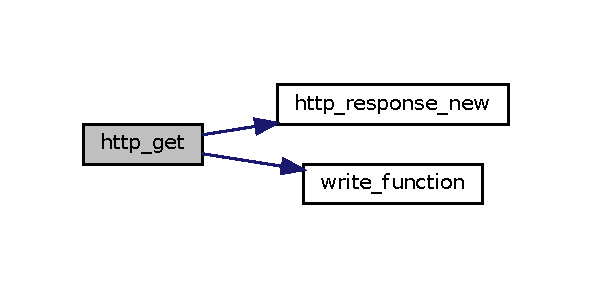
\includegraphics[width=284pt]{http_8c_a38c946ac3ac1ac192d43cb6595fdf5c3_cgraph}
\end{center}
\end{figure}
Here is the caller graph for this function\+:
\nopagebreak
\begin{figure}[H]
\begin{center}
\leavevmode
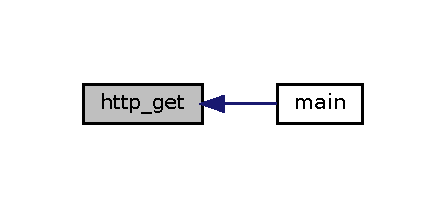
\includegraphics[width=214pt]{http_8c_a38c946ac3ac1ac192d43cb6595fdf5c3_icgraph}
\end{center}
\end{figure}
\mbox{\Hypertarget{http_8c_a47626df99e751c22b12fc185e4d84d7d}\label{http_8c_a47626df99e751c22b12fc185e4d84d7d}} 
\index{http.\+c@{http.\+c}!http\+\_\+response\+\_\+new@{http\+\_\+response\+\_\+new}}
\index{http\+\_\+response\+\_\+new@{http\+\_\+response\+\_\+new}!http.\+c@{http.\+c}}
\subsubsection{\texorpdfstring{http\+\_\+response\+\_\+new()}{http\_response\_new()}}
{\footnotesize\ttfamily \mbox{\hyperlink{struct_http_response}{Http\+Response}}$\ast$ http\+\_\+response\+\_\+new (\begin{DoxyParamCaption}{ }\end{DoxyParamCaption})}



Definition at line 20 of file http.\+c.



References Http\+Response\+::data, and Http\+Response\+::size.



Referenced by http\+\_\+get().


\begin{DoxyCode}
20                                   \{
21     \mbox{\hyperlink{struct_http_response}{HttpResponse}} * res = malloc(\textcolor{keyword}{sizeof}(\mbox{\hyperlink{struct_http_response}{HttpResponse}}));
22     res->\mbox{\hyperlink{struct_http_response_a11b910682b365528a15fcfd6d4dd824f}{size}} = 0;
23     res->\mbox{\hyperlink{struct_http_response_a29b7ecfb11da1af6c7fdd3fe7862901f}{data}} = malloc(res->\mbox{\hyperlink{struct_http_response_a11b910682b365528a15fcfd6d4dd824f}{size}}+1);
24     res->\mbox{\hyperlink{struct_http_response_a29b7ecfb11da1af6c7fdd3fe7862901f}{data}}[res->\mbox{\hyperlink{struct_http_response_a11b910682b365528a15fcfd6d4dd824f}{size}}] = \textcolor{charliteral}{'\(\backslash\)0'};
25     \textcolor{keywordflow}{return} res;
26 \};
\end{DoxyCode}
Here is the caller graph for this function\+:
\nopagebreak
\begin{figure}[H]
\begin{center}
\leavevmode
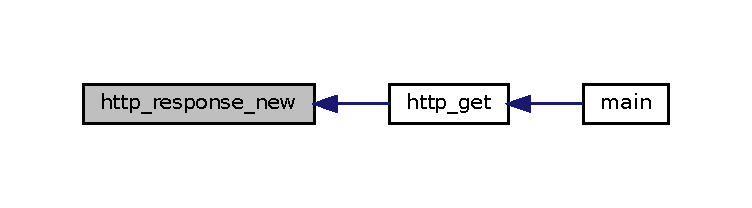
\includegraphics[width=350pt]{http_8c_a47626df99e751c22b12fc185e4d84d7d_icgraph}
\end{center}
\end{figure}
\mbox{\Hypertarget{http_8c_a4c00439adfc2c266dfc3f138a4bab5bb}\label{http_8c_a4c00439adfc2c266dfc3f138a4bab5bb}} 
\index{http.\+c@{http.\+c}!write\+\_\+function@{write\+\_\+function}}
\index{write\+\_\+function@{write\+\_\+function}!http.\+c@{http.\+c}}
\subsubsection{\texorpdfstring{write\+\_\+function()}{write\_function()}}
{\footnotesize\ttfamily size\+\_\+t write\+\_\+function (\begin{DoxyParamCaption}\item[{void $\ast$}]{ptr,  }\item[{size\+\_\+t}]{size,  }\item[{size\+\_\+t}]{nmemb,  }\item[{\mbox{\hyperlink{struct_http_response}{Http\+Response}} $\ast$}]{r }\end{DoxyParamCaption})}



Definition at line 12 of file http.\+c.



References Http\+Response\+::data, and Http\+Response\+::size.



Referenced by http\+\_\+get().


\begin{DoxyCode}
12                                                                             \{
13     \textcolor{keywordtype}{size\_t} new\_len = r->\mbox{\hyperlink{struct_http_response_a11b910682b365528a15fcfd6d4dd824f}{size}} + size*nmemb;
14     r->\mbox{\hyperlink{struct_http_response_a29b7ecfb11da1af6c7fdd3fe7862901f}{data}}= realloc(r->\mbox{\hyperlink{struct_http_response_a29b7ecfb11da1af6c7fdd3fe7862901f}{data}}, new\_len+1);
15     memcpy(r->\mbox{\hyperlink{struct_http_response_a29b7ecfb11da1af6c7fdd3fe7862901f}{data}}+r->\mbox{\hyperlink{struct_http_response_a11b910682b365528a15fcfd6d4dd824f}{size}}, ptr, size*nmemb);
16     r->\mbox{\hyperlink{struct_http_response_a29b7ecfb11da1af6c7fdd3fe7862901f}{data}}[new\_len] = \textcolor{charliteral}{'\(\backslash\)0'};
17     \textcolor{keywordflow}{return} size*nmemb;
18 \}
\end{DoxyCode}
Here is the caller graph for this function\+:
\nopagebreak
\begin{figure}[H]
\begin{center}
\leavevmode
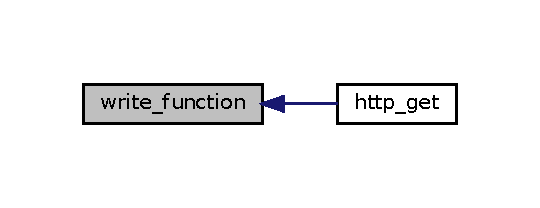
\includegraphics[width=336pt]{http_8c_a4c00439adfc2c266dfc3f138a4bab5bb_icgraph}
\end{center}
\end{figure}

%--- End generated contents ---

% Index
\backmatter
\newpage
\phantomsection
\clearemptydoublepage
\addcontentsline{toc}{chapter}{Index}
\printindex

\end{document}
